
\documentclass{beamer}


\mode<presentation>
{
  \usetheme{Singapore}
  \renewcommand{\insertnavigation}[1]{}
  \setbeamercovered{transparent}
}



\usepackage[english]{babel}
\usepackage[absolute,overlay]{textpos}
\usepackage[latin1]{inputenc}
\usepackage{times}
\usepackage{graphicx}
\usepackage{epstopdf}
\usepackage[T1]{fontenc}
\usepackage{soul}
\usepackage{pdflscape}
\usepackage{multirow}
\usepackage{pgf}
\usepackage{tikz}

\beamertemplatenavigationsymbolsempty

\newcommand{\citations}[1]
   {
     \begin{textblock}{16}[1,1](15.75,15.25)
       \flushright{\scriptsize #1}
     \end{textblock}
   }

\definecolor{MedPurple}{RGB}{194,165,207}
\definecolor{DeepPurple}{RGB}{118,42,131}
\definecolor{LightGreen}{RGB}{166,219,160}
\definecolor{DarkGreen}{RGB}{0,68,27}
\definecolor{MedGreen}{RGB}{90,174,97}

\setbeamercolor{title}{fg=DeepPurple}
\setbeamercolor{frametitle}{fg=DeepPurple}
\setbeamercolor{structure}{fg=DarkGreen}

\setbeamercolor{*}{bg=LightGreen}

\title[Specialisation \& the Latitude-niche-breadth Hypothesis]
{Specialisation \& the Latitude-niche-breadth Hypothesis}

\author[A.R. Cirtwill, D.B. Stouffer, \& T.N. Romanuk]{\textbf{Alyssa R. Cirtwill}, Daniel B. Stouffer, \& Tamara N. Romanuk} 
\institute[]
{
 %
  Stouffer Lab\\
  School of Biological Sciences\\
  University of Canterbury\\
  Christchurch, New Zealand\\
  ~\\
  www.stoufferlab.org\\
  %
}
\date[Short Occasion] 
{23 October 2015 | ABC 2015}

\subject{Talks}

\begin{document}

% \begin{frame}
%   \titlepage
% \end{frame}

\section*{Background}

  \begin{frame}{Testing the latitude-niche breadth hypothesis}

    \begin{center}
      \includegraphics*[width=.8\textwidth]{Figures/plant_richness.eps}

      \vspace{1cm}

    \textbf{Alyssa R. Cirtwill}\\ Daniel B. Stouffer \& Tamara N. Romanuk

    \vspace{1cm}

    23 October 2015 | ABC 2015

    \end{center}
  \end{frame}


  \begin{frame}{Testing the latitude-niche breadth hypothesis}

    \begin{center}
      \includegraphics*[width=.8\textwidth]{Figures/plant_richness.eps}

      \vspace{.5cm}

      Many groups are more diverse in the tropics\\
      \vspace{.5cm}
      {\color{white} Environmental stability? Productivity?\\}

      \vspace{1cm}

      {\color{white}23 October 2015 | ABC 2015}

    \end{center}
  \end{frame}


  \begin{frame}{Testing the latitude-niche breadth hypothesis}

    \begin{center}
      \includegraphics*[width=.8\textwidth]{Figures/plant_richness.eps}

      \vspace{.5cm}

      Many groups are more diverse in the tropics\\
      \vspace{.5cm}
      {\color{white}{Ey}}How?{\color{white}{Ey}}\\

      \vspace{1cm}

      {\color{white}23 October 2015 | ABC 2015}

    \end{center}
  \end{frame}


  \begin{frame}{Testing the latitude-niche breadth hypothesis}

    \begin{center}
      \includegraphics*[width=.8\textwidth]{Figures/plant_richness.eps}

      \vspace{.5cm}

      Many groups are more diverse in the tropics\\
      \vspace{.5cm}
      Environmental stability? Productivity?\\

      \vspace{1cm}

      {\color{white}23 October 2015 | ABC 2015}

    \end{center}
  \end{frame}


  \begin{frame}{Testing the latitude-niche breadth hypothesis}

    \begin{block}{Latitude-niche breadth version 1}
    \begin{center}
      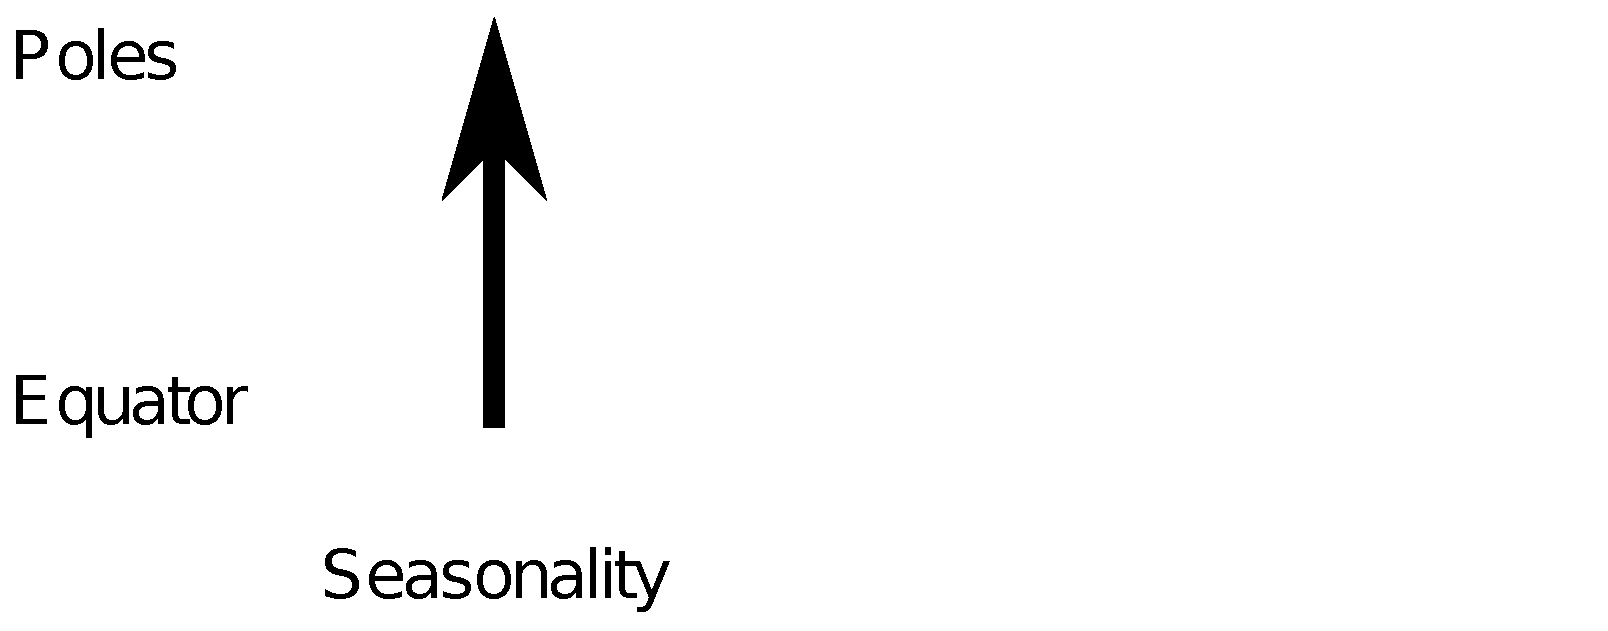
\includegraphics[width=.8\textwidth]{Figures/latitude_niche_breadth_1.eps}
    \end{center}

    \vspace{1cm}

    \tiny{Vazquez, D.P. \& Stevens, R.D. 2004. The latitudinal gradient in niche breadth: concepts and evidence. \emph{Am. Nat.}}
    \end{block}
  \end{frame}


  \begin{frame}{Testing the latitude-niche breadth hypothesis}

    \begin{block}{Latitude-niche breadth version 1}
    \begin{center}
      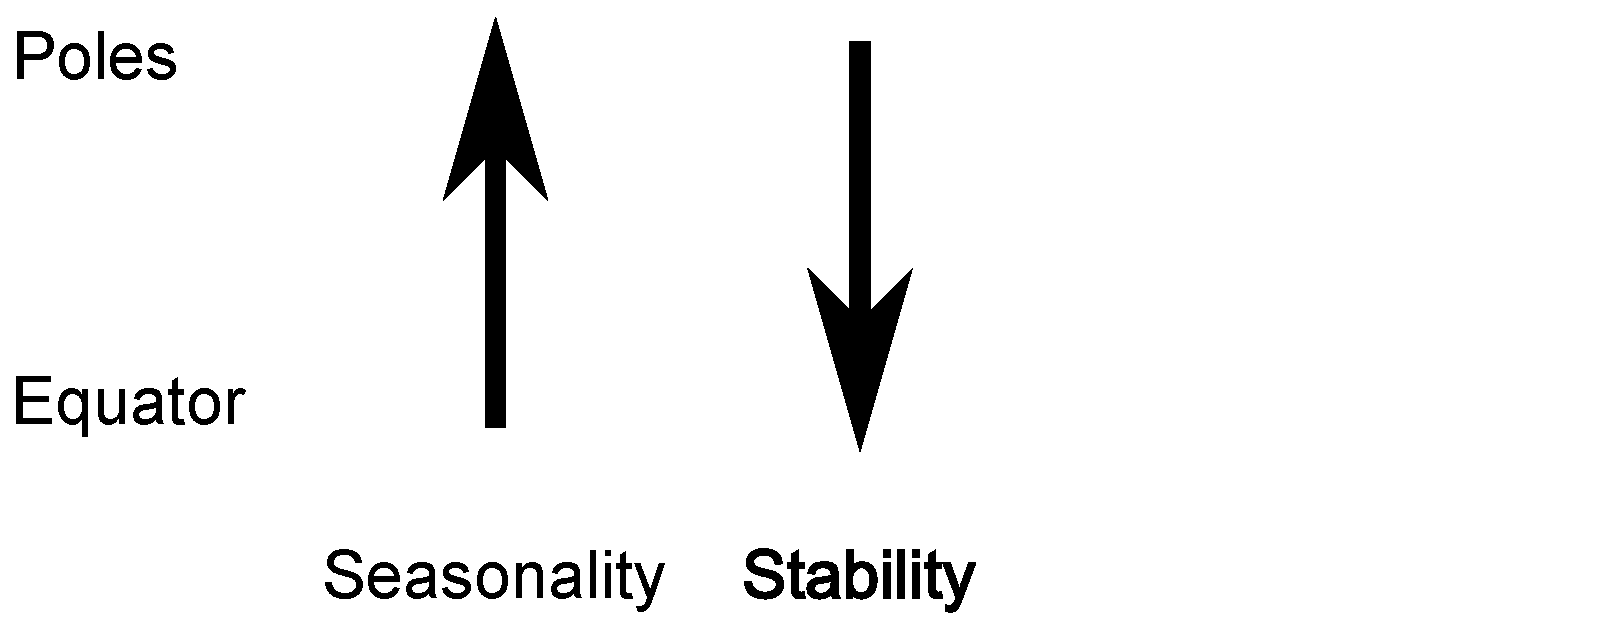
\includegraphics[width=.8\textwidth]{Figures/latitude_niche_breadth_2.eps}
    \end{center}

    \vspace{1cm}

    \tiny{Vazquez, D.P. \& Stevens, R.D. 2004. The latitudinal gradient in niche breadth: concepts and evidence. \emph{Am. Nat.}}
    \end{block}
  \end{frame}


  \begin{frame}{Testing the latitude-niche breadth hypothesis}

    \begin{block}{Latitude-niche breadth version 1}
    \begin{center}
      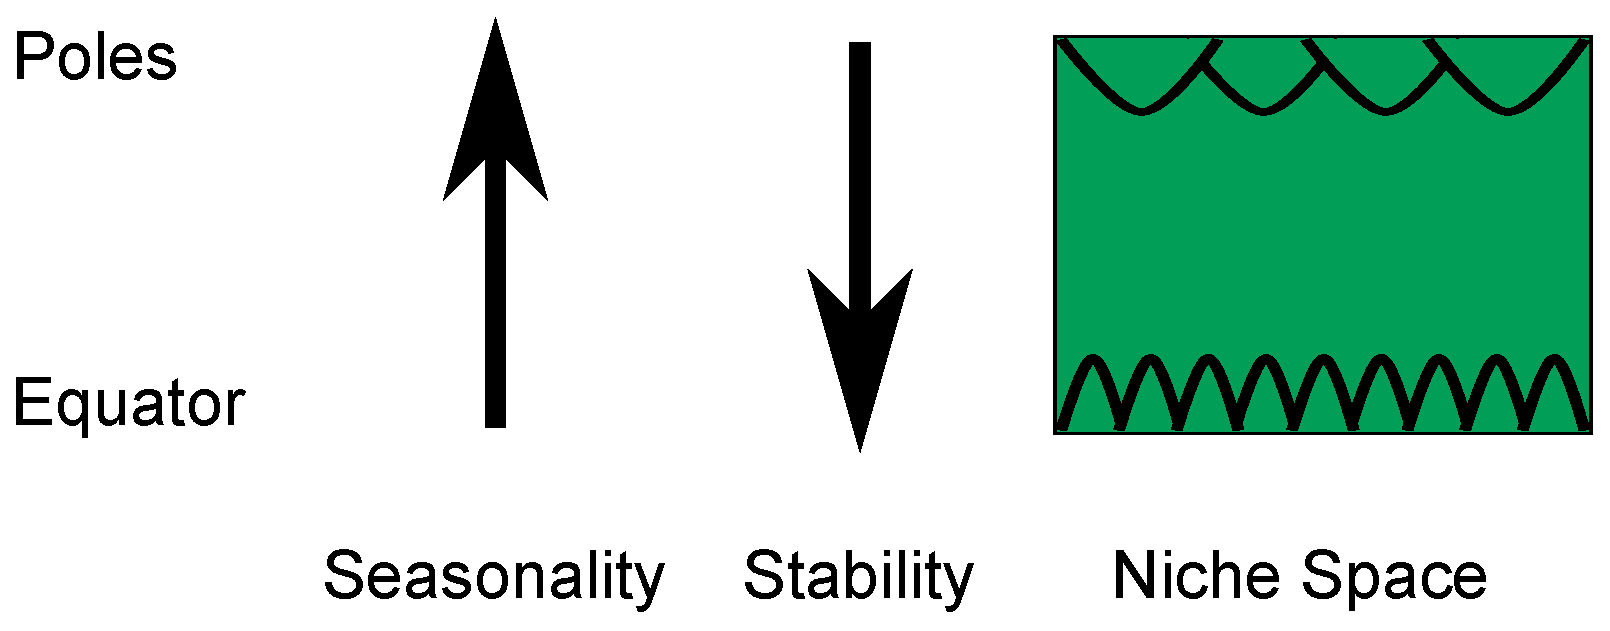
\includegraphics[width=.8\textwidth]{Figures/latitude_niche_breadth_3.eps}
    \end{center}

    \vspace{1cm}

    \tiny{Vazquez, D.P. \& Stevens, R.D. 2004. The latitudinal gradient in niche breadth: concepts and evidence. \emph{Am. Nat.}}
    \end{block}
  \end{frame}


  \begin{frame}{Testing the latitude-niche breadth hypothesis}
    \begin{block}{Latitude-niche breadth version 2}
    \begin{center}
      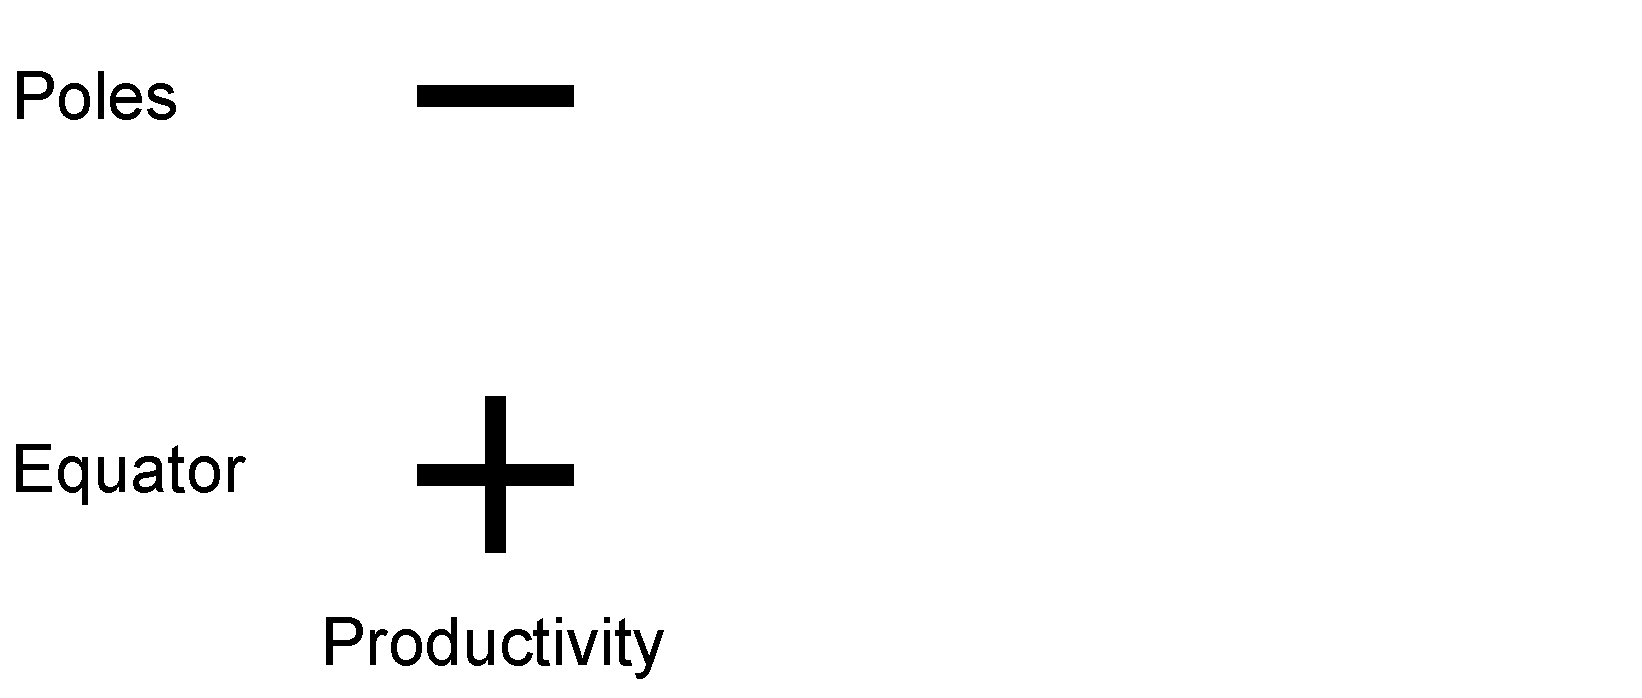
\includegraphics[width=.8\textwidth]{Figures/latitude_niche_breadth_4.eps}
    \end{center}

    \vspace{1cm}

    \tiny{Davies \emph{et. al.} 2007. Productivity alters the scale dependence of the diversity-invasibility relationship. \emph{Ecology.}}
    \end{block}
  \end{frame}


  \begin{frame}{Testing the latitude-niche breadth hypothesis}
    \begin{block}{Latitude-niche breadth version 2}
    \begin{center}
      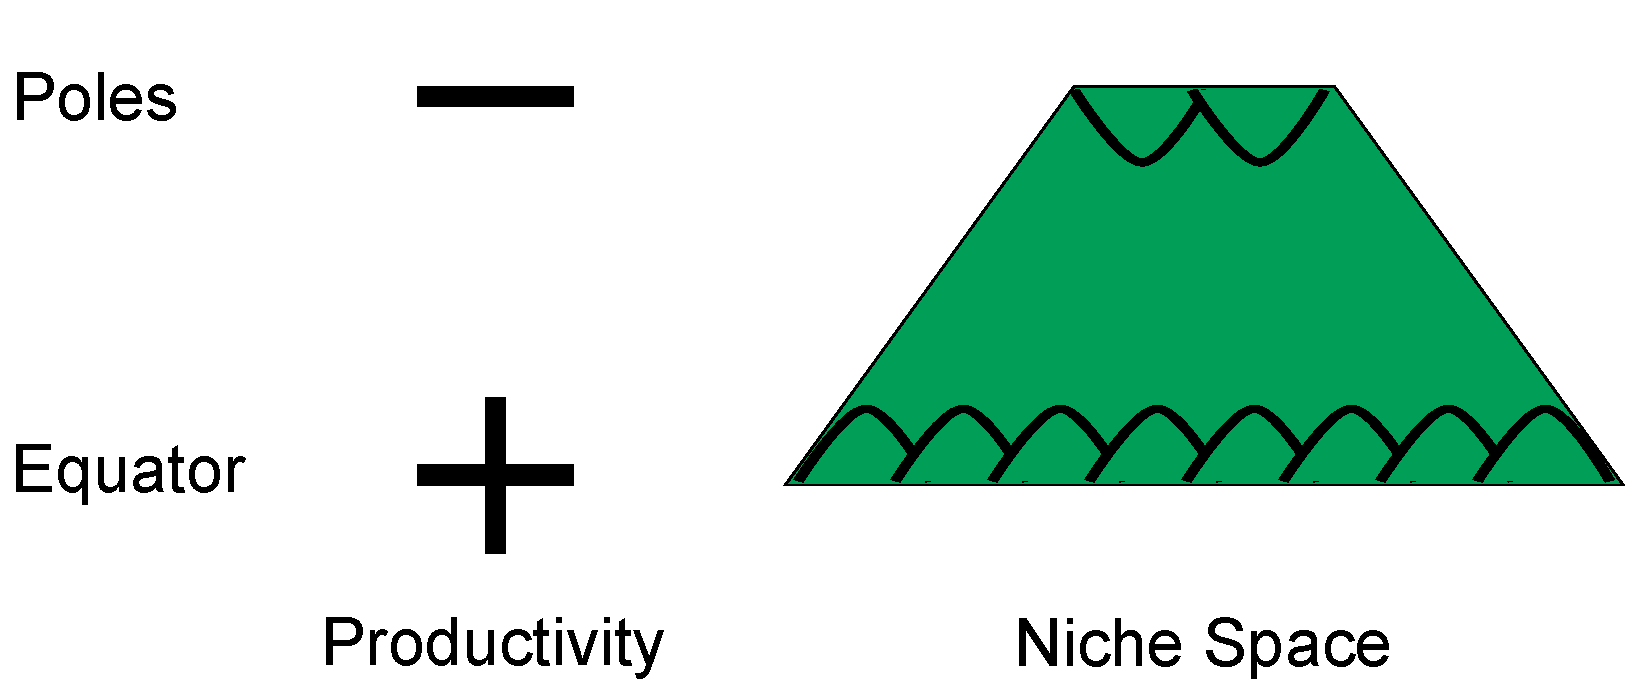
\includegraphics[width=.8\textwidth]{Figures/latitude_niche_breadth_5.eps}
    \end{center}

    \vspace{1cm}

    \tiny{Davies \emph{et. al.} 2007. Productivity alters the scale dependence of the diversity-invasibility relationship. \emph{Ecology.}}
    \end{block}
  \end{frame}


\section*{Food Webs}
  \begin{frame}{Testing the latitude-niche breadth hypothesis}
    \begin{columns}
    \column{.5in}
    \column{1.75in}
      \begin{center}
      \includegraphics[height=1in]{Figures/version1.eps}\\
      \vspace{.5cm}
      Greater specialisation\\in the tropics

      \vspace{.25cm}
      {\color{white}Fewer prey per species\\in the tropics}

      \end{center}
    \column{.5in}
    \column{1.75in}
      \begin{center}
      \includegraphics[height=1in]{Figures/version2.eps}\\
      \vspace{.5cm}
      Similar specialisation\\at all latitudes

      \vspace{.25cm}
      {\color{white}Equal prey per species\\at all latitudes}

      \end{center}
    \column{.5in}
    \end{columns}

    \vspace{.5cm}

    \begin{center}
      \color{white}{Generality : mean number of prey per species}
    \end{center}
  \end{frame}


  \begin{frame}{Testing the latitude-niche breadth hypothesis}
    \begin{columns}
    \column{.5in}
    \column{1.75in}
      \begin{center}
      \includegraphics[height=1in]{Figures/version1.eps}\\
      \vspace{.5cm}
      Greater specialisation\\in the tropics

      \vspace{.25cm}
      Fewer prey per species\\in the tropics

      \end{center}
    \column{.5in}
    \column{1.75in}
      \begin{center}
      \includegraphics[height=1in]{Figures/version2.eps}\\
      \vspace{.5cm}
      Similar specialisation\\at all latitudes

      \vspace{.25cm}
      Equal prey per species\\at all latitudes

      \end{center}
    \column{.5in}
    \end{columns}

    \vspace{.5cm}

    \begin{center}
      \color{white}{Generality : mean number of prey per species}
    \end{center}
  \end{frame}


  \begin{frame}{Testing the latitude-niche breadth hypothesis}
    \begin{columns}
    \column{.5in}
    \column{1.75in}
      \begin{center}
      \includegraphics[height=1in]{Figures/version1.eps}\\
      \vspace{.5cm}
      Greater specialisation\\in the tropics

      \vspace{.25cm}
      Lower generality\\in the tropics

      \end{center}
    \column{.5in}
    \column{1.75in}
      \begin{center}
      \includegraphics[height=1in]{Figures/version2.eps}\\
      \vspace{.5cm}
      Similar specialisation\\at all latitudes

      \vspace{.25cm}
      Equal generality\\at all latitudes

      \end{center}
    \column{.5in}
    \end{columns}

    \vspace{.5cm}

    \begin{center}
      \color{DarkGreen}{Generality : mean number of prey per species}
    \end{center}

  \end{frame}  


  \begin{frame}{Does niche breadth vary with latitude?}

    \begin{block}{Dataset}
    \begin{center}
      \includegraphics*[width=.75\textwidth]{Figures/LittleRockLake.eps}

      \vspace{.4cm}
    195 food webs \\
    5-188 species \\

    \end{center}
    \end{block}
  \end{frame}


  \begin{frame}{Does niche breadth vary with latitude?}

    \begin{block}{Dataset}
    \begin{center}
      \includegraphics*[width=.75\textwidth]{Figures/results/latitude_hist.eps}

    \end{center}
    \end{block}

  \end{frame}


  \begin{frame}{Does niche breadth vary with latitude?}

    \begin{block}{Dataset}
    \begin{center}
      \includegraphics*[width=.75\textwidth]{Figures/results/generality_hist.eps}

    \end{center}
    \end{block}

  \end{frame}


\section*{Scaling}
  \begin{frame}{Does niche breadth vary with latitude?}

    \begin{center}
      \includegraphics*[width=.8\textwidth]{Figures/results/Gen_vs_lat_simulated.eps}
    \end{center}

  \end{frame}


  \begin{frame}{Niche breadth scales with species richness}

    \begin{center}
      \includegraphics*[width=.654\textwidth]{Figures/results/Gen_dots_vs_S_fitline_observed.eps}

    \vspace{.3cm}
      {\Large      
      $G \approx aS^b$}
    \end{center}
  \end{frame}

  \begin{frame}{Niche breadth scales with species richness}

    \begin{center}
      \includegraphics*[width=.654\textwidth]{Figures/results/Gen_dots_vs_S_fitline_observed.eps}

    \vspace{.3cm}
      {\Large      
      log($G$) $\approx b$  log($a$)  log($S$) }
    \end{center}
  \end{frame}


 \begin{frame}{Niche breadth scales with species richness}

    \begin{center}
      \includegraphics*[width=.654\textwidth]{Figures/results/Gen_vs_lat_negative.eps}

    \vspace{.3cm}
      {\Large      
      $G \approx aS^b$ \hspace{.5in} $S \approx Latitude$}
    \end{center}

  \end{frame}


  \begin{frame}{Does latitude affect scaling of niche breadth?}

    \begin{center}
      \includegraphics*[width=.654\textwidth]{Figures/results/Gen_dots_vs_S_fitline_observed.eps}

    \vspace{.3cm}
      {\Large      
      $G \approx aS^b$}
    \end{center}
  \end{frame}


  \begin{frame}{Does latitude affect scaling of niche breadth?}

    \begin{center}
      \includegraphics*[width=.654\textwidth]{Figures/results/Gen_dots_vs_S_fitline_observed.eps}

    \vspace{.3cm}
      {\Large      
      $G \approx aS^{\color{DeepPurple}b}$}
    \end{center}
  \end{frame}


  \begin{frame}{Does latitude affect scaling of niche breadth?}
    \begin{center}
      \includegraphics*[width=.654\textwidth]{Figures/results/Gen_dots_vs_S_fitline_observed.eps}

      \vspace{.3cm}
      {\Large
      $G \approx aS^{\color{DeepPurple}b_0+b_1Latitude}$}
    \end{center}
  \end{frame}


  \begin{frame}{Does latitude affect scaling of niche breadth?}
    \begin{center}
      \includegraphics*[width=.654\textwidth]{Figures/results/Gen_vs_S_expectations.eps}

      \vspace{.3cm}
      {\Large
      $G \approx aS^{\color{DeepPurple}b_0+b_1Latitude}$}
    \end{center}
  \end{frame}


\section*{Results}
  \begin{frame}{Does latitude affect scaling of niche breadth?}
    \begin{center}
      \includegraphics*[width=.9\textwidth]{Figures/results/Gen_vs_S_marginal_axis.eps}

      \vspace{.3cm}
      {\Large
      $G \approx aS^{\color{DeepPurple}b_0+b_1Latitude}$}

    \end{center}
  \end{frame}


  \begin{frame}{Does latitude affect scaling?}
    \begin{center}
      \includegraphics*[width=.9\textwidth]{Figures/results/Gen_vs_S_marginal_one.eps}

      \vspace{.3cm}
      {\Large
      $G \approx aS^{\color{DeepPurple}b_0+b_1Latitude}$}

    \end{center}
  \end{frame}


  \begin{frame}{Does latitude affect scaling?}
    \begin{center}
      \includegraphics*[width=.9\textwidth]{Figures/results/Gen_vs_S_marginal.eps}

      \vspace{.3cm}
      {\Large
      $G \approx aS^{\color{DeepPurple}b_0+b_1Latitude}$}

    \end{center}
  \end{frame}


\section*{Discussion}

  \begin{frame}{Estuarine, Marine, \& Terrestrial Food Webs}
    \begin{center}
      \includegraphics*[width=.9\textwidth]{Figures/results/no_effect.eps}

    \vspace{.5cm}

    \includegraphics*[width=.75\textwidth]{Figures/results/no_effect_interpretations.eps}

    \end{center}
  \end{frame}


  \begin{frame}{Estuarine, Marine, \& Terrestrial Food Webs}
    \begin{center}
      \includegraphics*[width=.9\textwidth]{Figures/results/no_effect.eps}

    \vspace{1.02cm}

    \includegraphics*[width=.4\textwidth]{Figures/version2.eps}

    \end{center}
  \end{frame}


  \begin{frame}{Lake \& Stream Food Webs}
    \begin{center}
      \includegraphics*[width=.75\textwidth]{Figures/results/effect.eps}

      \vspace{.5cm}

    \includegraphics*[width=.75\textwidth]{Figures/results/effect_interpretations.eps}

    \end{center}
  \end{frame}


  \begin{frame}{Lake \& Stream Food Webs}
    \begin{center}
      \includegraphics*[width=.75\textwidth]{Figures/results/effect.eps}

    \vspace{1.02cm}

    \includegraphics*[width=.255\textwidth]{Figures/version1.eps}

    \end{center}
  \end{frame}


\section*{Freshwaters}

  \begin{frame}{How do lakes and streams differ}
    \begin{block}{from terrestrial food webs?}

      \begin{columns}
        \column{.5in}
      
        \column{1.9in}
          \begin{center}
          \includegraphics[width=.8\textwidth]{Figures/anteater.eps}
          \end{center}
        \column{.2in}
        \column{1.9in}
          \begin{center}
          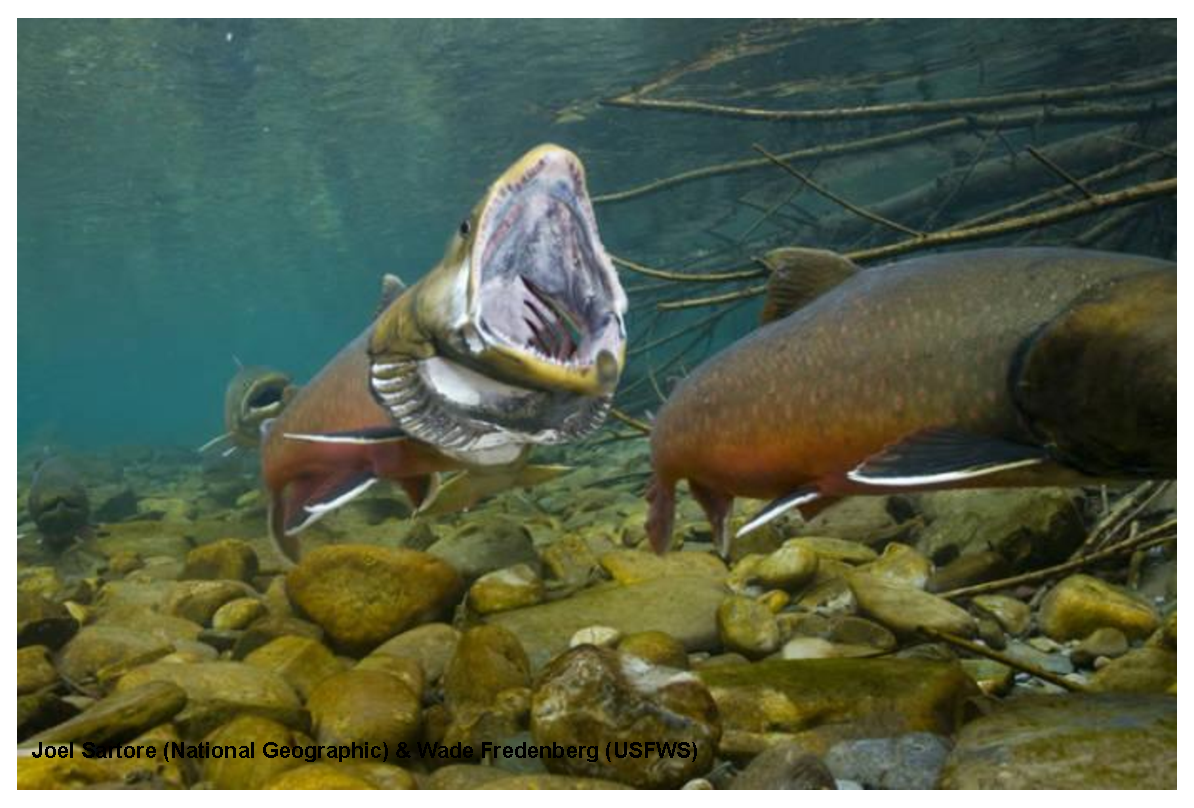
\includegraphics[width=.8\textwidth]{Figures/trout.eps}
          \end{center}
        \column{.5in}
      \end{columns}

        \vspace{.5cm}

      \begin{columns}
        \column{.5in}
      
        \column{1.9in}

         \begin{center}
        
        Gape-limitation!

        \vspace{.25cm}

        {\tiny Liem 1990, \emph{Am. Zool}}\\
        {\tiny Shurin \emph{et. al.} 2007, \emph{Ecol. Lett.}}
        \end{center}

        \column{.2in}

        \column{1.9in}

          \begin{center}
          \includegraphics[width=.5\columnwidth]{Figures/version1.eps}
          
          \end{center}  

        \column{.5in}

      \end{columns}
    \end{block}
  \end{frame}

  \begin{frame}{How do lakes and streams differ}
    \begin{block}{from estuarine \& marine food webs?}

      \begin{columns}
        \column{.5in}
        \column{1.9in}

        \hfill \includegraphics[width=.8\columnwidth]{Figures/spring_stream.eps}

        \vspace{.2in}

        \hfill \includegraphics[width=.8\columnwidth]{Figures/fall_stream.eps}

        \column{.2in}

        \column{1.9in}

        \includegraphics[width=.8\columnwidth]{Figures/summer_stream.eps}

        \vspace{.2in}

        \includegraphics[width=.8\columnwidth]{Figures/winter_stream.eps}

        \column{.5in}

      \end{columns}
    \end{block}

    \vfill

  \end{frame}

\section*{Conclusion and Acknowledgements}
  \begin{frame}{Evidence for the latitude-niche breadth hypothesis}
    \begin{block}{Estuarine, marine, \& terrestrial webs}
      \begin{columns}
      \column{2.5in}
        \begin{itemize}
          \item Broader niche space\\ in the tropics
          \item Similar specialisation\\ everywhere
        \end{itemize}
      \column{1in}

        \begin{center}

        \includegraphics[height=.75in]{Figures/version2.eps}

        \end{center}

      \column{.5in}
      \end{columns}
    \end{block}

    \begin{block}{Lake \& stream webs}
      \begin{columns}
      \column{2.5in}
      \begin{itemize}
        \item Narrower niches\\ in the tropics
        \item Specialisation\\ due to stability?
      \end{itemize}
      \column{1in}

        \begin{center}
      
        \includegraphics[height=.75in]{Figures/version1.eps}
      
        \end{center}
      
      \column{.5in}
    \end{columns}
    \end{block}
  \end{frame}

  \begin{frame}{Acknowledgements}
    \begin{columns}
      \column{.25in}

      \column{1.5in}
      \centering

      Daniel B. Stouffer\\
      \& his lab
      
      \column{1.5in}
      \centering

      Tamara N. Romanuk\\
      \& her lab

      \column{1.5in}
      \centering

      Angus McIntosh\\
      Matthias Schleuning

      \column{.25in}
    \end{columns}

    \vspace{.5cm}

    \begin{columns}
    \column{.25in}
     \column{2.25in}
       \centering

      
\includegraphics[height=.75in]{marsden-logo-cmyk-tif.eps}

      \vspace{.5cm}
      \vspace{.125in}

      
\includegraphics[height=.5in]{Dal_logo.eps}

      \vspace{.125in}

     \column{2.25in}
       \centering

       \includegraphics[height=.75in]{NSERC_C.eps}

       \vspace{.5cm}

       
\includegraphics[height=.75in]{logo-canterbury-color.eps} 

    \column{.25in}
    \end{columns}
  \end{frame}

  \begin{frame}{Evidence for the latitude-niche breadth hypothesis}

    \begin{columns}
    \column{.5in}
    \column{2.75in}
      \begin{center}
      \includegraphics[height=.8in]{Figures/results/no_effect.eps}
      \end{center}


    \column{.25in}
    \column{1in}
      \begin{center}

        \includegraphics[height=.65in]{Figures/version2.eps}
        \vspace{.3in}

      \end{center}

    \column{.5in}
    \end{columns}

    \begin{columns}
    \column{.5in}
    \column{2.75in}
      \begin{center}

      \includegraphics[height=.8in]{Figures/results/effect.eps}
      \end{center}

    \column{.25in}
    \column{1in}
      \begin{center}

        \includegraphics[height=.65in]{Figures/version1.eps}
        \vspace{.3in}

      \end{center}

    \column{.5in}
    \end{columns}


    \vspace{.1in}

    \begin{center}

    {\Large $G \approx aS^{\color{DeepPurple}b_0+b_1Latitude}$}

    \end{center}

  \end{frame}




\end{document}
